\section{House Model R and C Values}

In heat transfer theory the basic thermal circuit contains thermal resistances. Heat transfer occurs via conduction, convection and radiation. In analogy with Ohm's Law for electricity, expressions can be derived for the heat transfer rate (analogous to electrical current) and the thermal resistances (analogous to ohmic resistances) in these three modes of heat transfer. The temperature difference plays a role analogous to the electrical voltage difference. These expressions are shown in Fig. \ref{fig:htr}.
\begin{figure}[H]
	\centering
	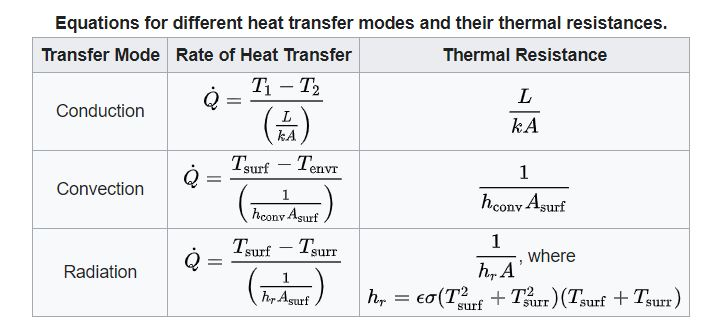
\includegraphics[width=0.8\columnwidth]{Pictures/heat transfer mode.JPG}
	\caption[Short title]{Heat transfer model \cite{GIGO}}.
	\label{fig:htr}
\end{figure}

In \cite{HTTHERMO} and \cite{FUND} the expressions in Fig. \ref{fig:htr} are derived.
For conduction, the expression for $R_{th} = \frac{L}{k\dot A}$

$L$ is the distance over which heat transfer takes place, or the thickness of the material
$A$ is the conductive surface area

The units of $R_{th}$ are: $ [\frac{K}{W}] $

$ [W] = [\frac{W}{m \cdot K}] \dot [m^2] \cdot [\frac{K}{m}] $

The units of $k$ are: $ [\frac{m}{m^2} \cdot \frac{W}{K}] = [\frac{W}{m \cdot K}]$

Thermal conductivity of material $k = [\frac{W}{m \cdot K }] = [\frac{W}{m \cdot K }]  = [W \cdot m^{-1} \cdot K^{-1}]$

$k$ is also denoted as $\lambda$

Reference: \cite{ELECRESCOND}

Ohm's Law: $ R = \frac{U}{I} \quad [\frac{V}{A}] = [\Omega] $

Electrical resistivity: $ \rho = [\frac{\Omega \cdot m^2}{m} ] = [\Omega \cdot m] $ Material property.

Electrical conductivity: $ \sigma = \frac{1}{\rho} =[\frac{1}{\Omega \cdot m}] = [\frac{S}{m}] $ Material property.

Electrical resistance $ R = \frac{\rho \cdot L}{A} $ or $ R = \frac{L}{\sigma \cdot A} $
\\

Thermal Law: 
Heat flux $ \dot Q $ in $ [W \cdot m^{-2}] $

$ \dot Q = \frac{\Delta T}{R_{th}} \quad R_{th} = \frac{\Delta T}{\dot  Q} 
\quad [\frac{K}{W \cdot m^{-2}}] = [\frac{m^2 \cdot K}{W}]$

(Specific) Thermal resistivity: $ R_\lambda $ or $ r = [\frac{K}{W \cdot m^{-2}} \frac{1}{m} ] = [\frac{m \cdot K}{W}] $ Material property.

Thermal conductivity: $ \lambda $ or $ k  = \frac{1}{r} = [\frac{ W \cdot m^{-2} }{K} \cdot m] 
= [\frac{W}{m \cdot K}] $ Material property

Thermal resistance R-value or $ R_{th} = \frac{r \cdot L}{A} $ or $ R = \frac{L}{k \cdot A} $

Unit $ R_{th} = [\frac{m \cdot K}{W} \frac{m}{m^2}] = [\frac{m^2 \cdot K}{W}] $
\\

$R_c$-value $ = r \cdot L = \frac{L}{k} = \frac{L}{\lambda} $
\\

Some typical heat transfer thermal resistance values, also denoted as R\textsubscript{c}-values are: \cite{OVERALL}: 

\begin{itemize}
	\item Static layer of air, 40 mm thickness (1.57 in)  : R = 0.18 [$m^2K/W$].
	\item Inside heat transfer resistance, horizontal current : R = 0.13 [$m^2k/W$]. 
	\item Outside heat transfer resistance, horizontal current : R = 0.04 [$m^2K/W$].
	\item Inside heat transfer resistance, heat current from down upwards : R = 0.10 [$m^2K/W$].
	\item Outside heat transfer resistance, heat current from above downwards : R = 0.17 [$m^2K/W$].
	
\end{itemize}

\begin{figure}[H]
	\centering
	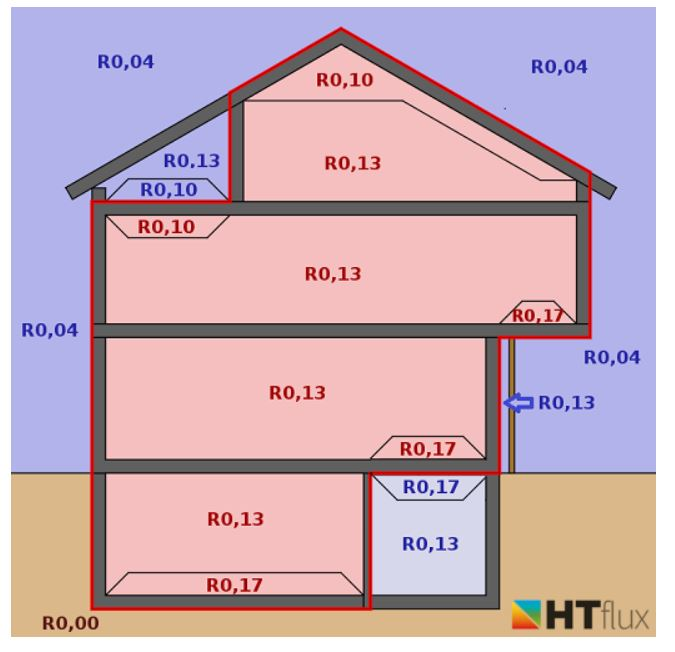
\includegraphics[width=0.8\columnwidth]{Pictures/Overview of heat resistances.JPG}
	\caption[Short title]{An overview of heat transfer resistance \cite{SURFREST}.}
	\label{fig:overview}
\end{figure}


The standard R\textsubscript{c}-values that have been used for facades, roof and floor until 2020 are summarized in Fig. \ref{fig:Rc}:

\begin{figure}[H]
	\centering
	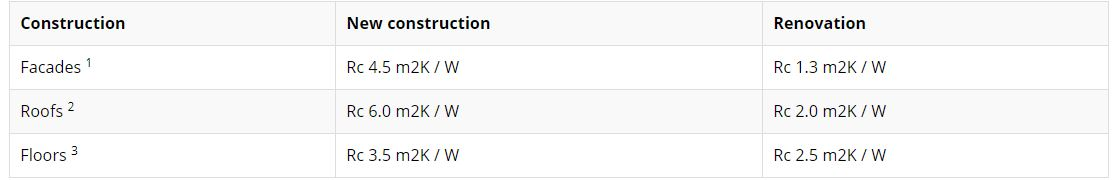
\includegraphics[width=1.0\columnwidth]{Pictures/Rc_values_2020.JPG}
	\caption[Short title]{Rc Values \cite{ISOL}}
	\label{fig:Rc}
\end{figure}

New standard values will be used from 1-1-2021, since the building standard NEN 1068 will be replaced by the NTA 8800 standard. The old and new situation is described in "EnergieVademecum Energiebewust ontwerpen van nieuwbouwwoningen", chapter 5: Thermische isolatie, thermische bruggen en luchtdichtheid.
\cite{ISSO}.

\begin{figure}[H]
	\centering
	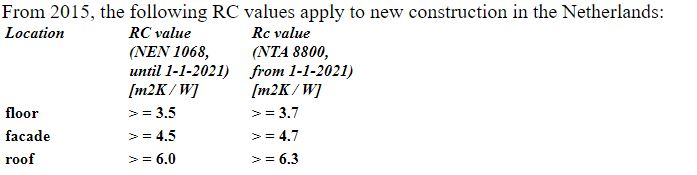
\includegraphics[width=1.0\columnwidth]{Pictures/Rc_values_2021.JPG}
	\caption[Short title]{Rc Values \cite{RVALUE}}
	\label{fig:newRc}
\end{figure}

The values used for different types of houses such as: row houses, detached houses and apartments can be found in the document "Voorbeeldwoningen 2011" \cite{VOORBEELD}. An example with values for a common type of row house, built in the period from 1975 to 1991 is shown in Fig. \ref{fig:rowhouse}:


\begin{figure}[H]
	\centering
	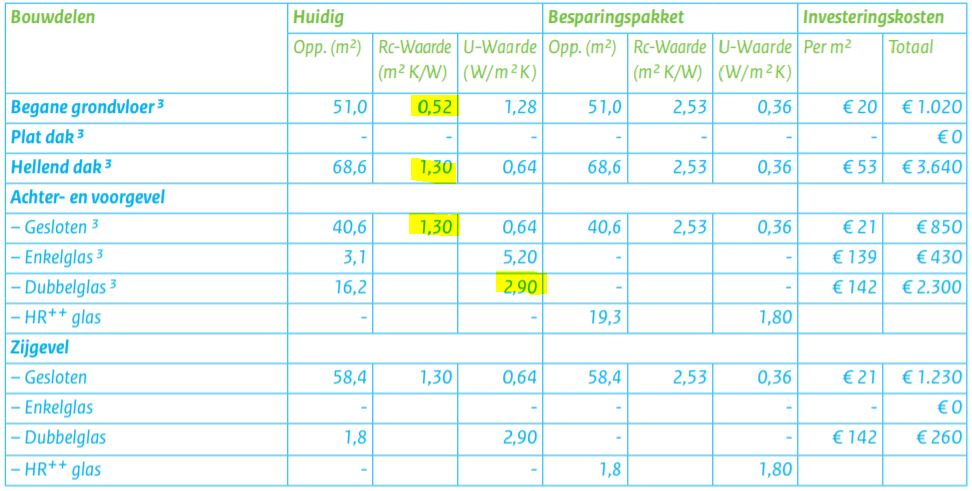
\includegraphics[width=0.8\columnwidth]{Pictures/row_house_1975-1991.JPG}
	\caption[Short title]{R\textsubscript{c}-values for a row house type built between 1975-1991 \cite{VOORBEELD}}
	\label{fig:rowhouse}
\end{figure} 

%\newpage
